%!TEX root = ../my_thesis.tex
\section[$\Bz\to\Dmp\pipm$ selection studies]{\boldmath{$\Bz\to\Dmp\pipm$} selection studies}
\label{app:selectionStudies}

\subsection{BDT input features}
\label{app:BDTinput}
The distributions of the input features for the BDT (listed and defined in Table~\ref{tab:BDTinput})
are shown in Figs.~\ref{fig:BDTinput1}, \ref{fig:BDTinput2} and \ref{fig:BDTinput3}.

\begin{figure}[htpb]
  \begin{center}
    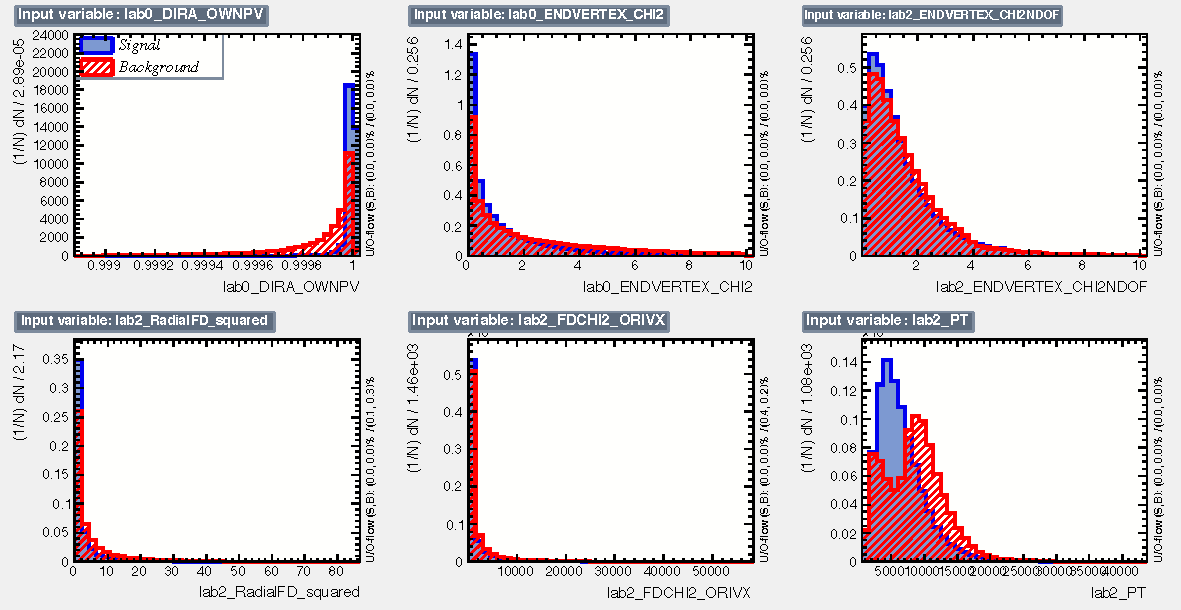
\includegraphics[width=\textwidth]{AA-Appdx-selection/figs/variables_id_c1.pdf}
  \end{center}
  \vspace{-2mm}
  \caption{Input features used in the BDT training. From top left to bottom right: cosine of the direction angle of
  		the \Bz, $\chi^2$ of the $\Bz$ vertex, $\chi^2/\text{ndof}$ of the $\Dmp$ vertex, $\Dmp$ radial flight
  		distance, $\Dmp$ flight distance $\chi^2$ with respect to the $\Bz$ vertex and transverse momentum of the $\Dmp$.}
  \label{fig:BDTinput1}
\end{figure}
\begin{figure}[t]
  \begin{center}
    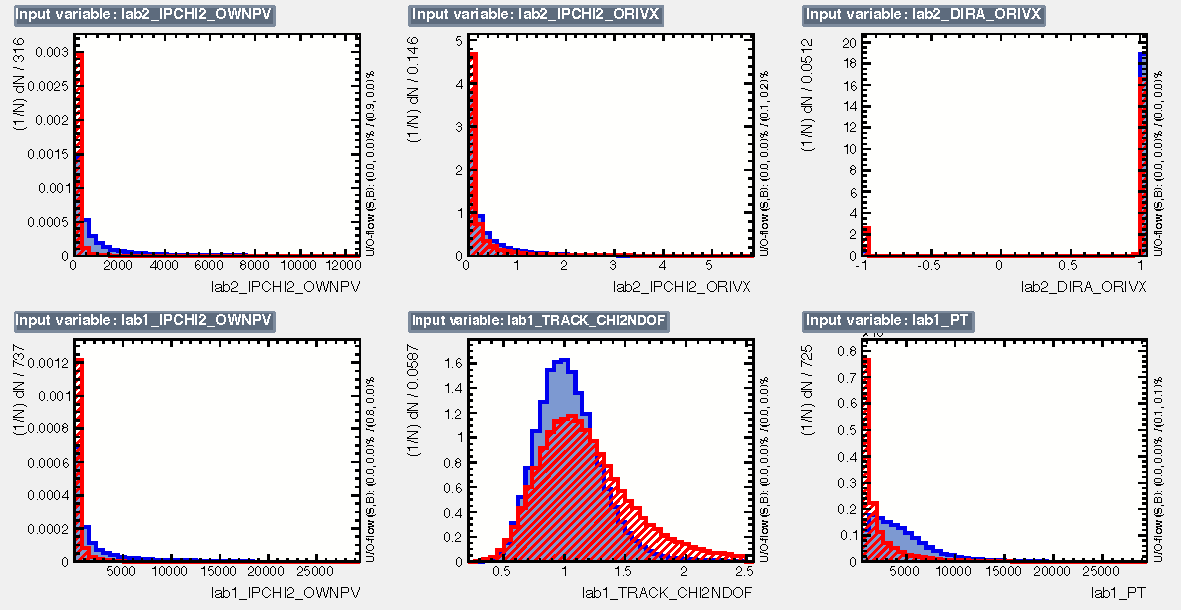
\includegraphics[width=\textwidth]{AA-Appdx-selection/figs/variables_id_c2.pdf}
  \end{center}
  \vspace{-2mm}
  \caption{Input features used in the BDT training. From top left to bottom right: $\Dmp$ $\text{IP}\chi^2$ with respect to the associated
  		PV and the $\Bz$ vertex, cosine of the direction angle of the $\Dmp$, the $\text{IP}\chi^2$ with respect to the associated PV of the
  		bachelor pion, track $\chi^2/\text{ndof}$ of the bachelor pion and the transverse momentum of the bachelor pion.}
  \label{fig:BDTinput2}
\end{figure}
\begin{figure}[t]
  \begin{center}
    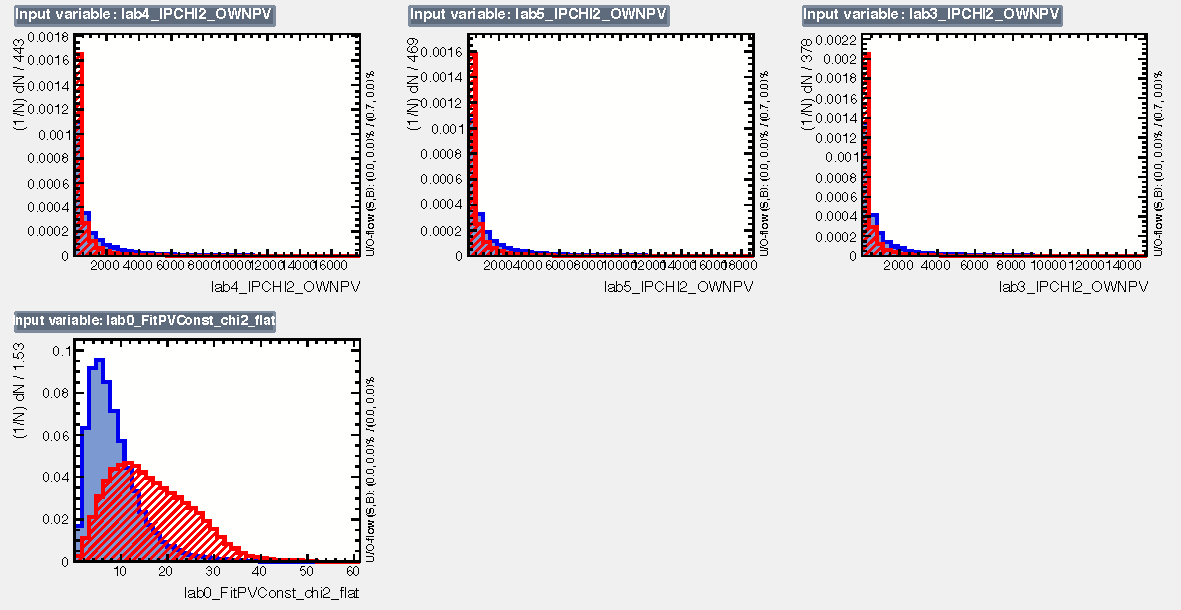
\includegraphics[width=\textwidth]{AA-Appdx-selection/figs/variables_id_c3.pdf}
  \end{center}
  \vspace{-2mm}
  \caption{Input features used in the BDT training. From top left to bottom right: $\text{IP}\chi^2$ of the associated primary
  		vertex of the three $\Dmp$ daughters and the $\chi^2$ of the decay tree fit with PV constraint.}
  \label{fig:BDTinput3}
\end{figure}

\subsection{Multiple candidates}
\label{app:multiplecandidates}

Table~\ref{tab:multibeforesel} gives a summary of the multiple candidates left after stripping and trigger selection, while Table~\ref{tab:multiaftersel} 
reports the number of multiple candidates after stripping, trigger and offline selection.

\begin{table}[htbp]
%\footnotesize
  \centering
  \caption{Statistical information on multiple $\Bz\to\Dmp\pipm$ candidates left after stripping and trigger selection.}
    \begin{tabular}{lcccc}
    \toprule
      & \multicolumn{2}{c}{2011} & \multicolumn{2}{c}{2012}\\
    \midrule
     fraction of candidates that & \multicolumn{2}{c}{\multirow{2}[2]{*}{\SI{18.3}{\percent}}} & \multicolumn{2}{c}{\multirow{2}[2]{*}{\SI{19.5}{\percent}}}\\
     are not unique in a given event & & & & \\
    \midrule
    fraction of candidates to be discarded & \multicolumn{2}{c}{\multirow{2}[2]{*}{\SI{10.1}{\percent}}} & \multicolumn{2}{c}{\multirow{2}[2]{*}{\SI{11.0}{\percent}}}\\
       to maintain one candidate per event & & & & \\
    \midrule
    fraction of events with & \multicolumn{2}{c}{\multirow{2}[2]{*}{\SI{9.0}{\percent}}} & \multicolumn{2}{c}{\multirow{2}[2]{*}{\SI{9.6}{\percent}}}\\
    multiple  candidates & & & & \\
    \cmidrule(r){2-5}
      & \#cands & \#events & \#cands & \#events\\
      \cmidrule(r){2-5}
      & 1 & 5940804 & 1 & 16407228\\
      & 2 & 483991  & 2 & 1426286\\
      & 3 & 73902    & 3 & 226205\\
      & 4 & 20093     & 4 & 62640\\
      & 5 & 6132      & 5 & 19213\\
      & 6 & 2505      & 6 & 8044\\
      & 7 & 1087      & 7 & 3326\\
      & 8 & 528      & 8 & 1686\\
      & 9 & 251      & 9 & 839\\
      & 10 & 146      & 10 & 461\\
      & 11 & 78      & 11 & 279\\
      & 12 & 40      & 12 & 178\\
      & 13 & 28      & 13 & 109\\
      & 14 & 32      & 14 & 85\\
      & 15 & 10      & 15 & 53\\
      & 16 & 12      & 16 & 24\\
      & 17 & 7      & 17 & 16\\
      & 18 & 4      & 18 & 20\\
      & 19 & 5      & 19 & 9\\
      & 20 & 1      & 20 & 11\\
      & 21 & 3      & 21 & 5\\
      & 22 & 2      & 22 & 3\\
      & 23 & 0      & 23 & 2\\
      & 24 & 2      & 24 & 2\\
      & 25 & 1      & 25 & 1\\
      & 26 & 0      & 26 & 4\\
      & 30 & 0      & 30 & 1\\
      & 33 & 0      & 33 & 1\\
      & 40 & 1      & 40 & 0\\
      & 41 & 0      & 41 & 1\\
      \bottomrule
    \end{tabular}
    \label{tab:multibeforesel}
\end{table}
\begin{table}[!phtb]
\centering
\caption{
Statistical information on multiple $\Bz\to\Dmp\pipm$ candidates left after stripping, trigger and offline selection.}
\begin{tabular}{lcccc}
\toprule
 & \multicolumn{2}{c}{2011} & \multicolumn{2}{c}{2012}\\
\midrule
fraction of candidates pairs & \multicolumn{2}{c}{\multirow{2}[2]{*}{\SI{0.8}{\percent}}} & \multicolumn{2}{c}{\multirow{2}[2]{*}{\SI{0.8}{\percent}}}\\
that are not unique in an event & & & & \\
\midrule
fraction of candidates to be discarded & \multicolumn{2}{c}{\multirow{2}[2]{*}{\SI{0.4}{\percent}}} & \multicolumn{2}{c}{\multirow{2}[2]{*}{\SI{0.4}{\percent}}}\\
to maintain one candidate per event & & & & \\
\midrule
fraction of events with & \multicolumn{2}{c}{\multirow{2}[2]{*}{\SI{0.4}{\percent}}} & \multicolumn{2}{c}{\multirow{2}[2]{*}{\SI{0.4}{\percent}}}\\
multiple candidates & & & & \\
\cmidrule(r){2-5}
 & \#cands & \#events & \#cands & \#events\\
\cmidrule(r){2-5}
 & 1 & 483074 & 1 & 1200956\\
 & 2 & 1886   & 2 & 4962\\
 & 3 & 38     & 3 & 98\\
 & 4 & 4      & 4 & 9\\
 & 5 & 1      & 5 & 3\\
\bottomrule
\end{tabular}
\label{tab:multiaftersel}
\end{table}
